\documentclass{article}

\title{Programación de modelos físico-matemáticos con FORTRAN 90}
\author{Borja del Campo López \and Imanol Sardón Delgado}
\date{28 de enero de 2019}
\usepackage[margin=1in]{geometry}
\usepackage{graphicx}
\usepackage{pdfpages}
\usepackage[hidelinks]{hyperref}

\begin{document}
	
	\maketitle
	\thispagestyle{empty}
%	\includepdf[pages=1-2]{Enunciado}
	\newpage
	\tableofcontents
	\newpage
	
	\section{Introducción}
	
	Para llegar a un producto final en lo referente a modelos físico-matemáticos se tiene que seguir una secuencia bien definida de pasos que se muestran en la siguiente figura.
	
	\begin{figure}[h!]
		\begin{center}
			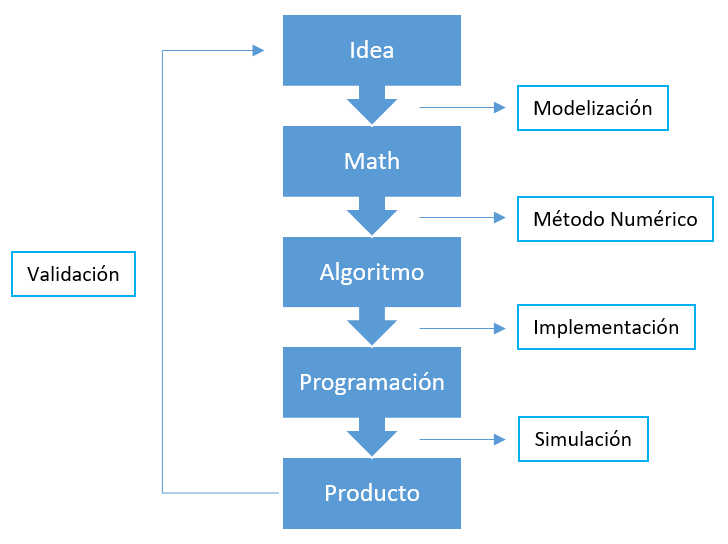
\includegraphics[scale=0.7]{sequence.png}
			\caption{Secuencia para la obtención de un producto de programación de un modelo físico-matemático}
		\end{center}
	\end{figure}

	En primer lugar, todo empieza con una idea de lo que se quiere lograr. En este punto de la secuencia se puede decir que "cabe todo", es decir, la idea puede ser completamente ambiciosa e innovadora. Mediante la modelización se llega a un modelo matemático de la idea que se ha definido previamente. Es en este momento cuando la idea va aterrizando poco a poco y se empieza a ver qué cosas de las inicialmente propuestas en el momento de la creación de la idea son factibles y cuáles no lo son. Posteriormente, aparece la necesidad de resolver el problema matemático que ha surgido del paso anterior. En la gran mayoría de problemas que aparecen en la realidad, la matemática es demasiado compleja como para obtener una solución analítica. Por eso se hace necesario el empleo de métodos numéricos para la obtención de soluciones. Una vez se ha elegido un método numérico y se ha aplicado al modelo matemático se obtiene un algoritmo, es decir, una secuencia finita de instrucciones con el objetivo de alcanzar la solución del problema planteado. El siguiente paso consiste en la implementación de este algoritmo mediante un lenguaje de programación para obtener una aplicación informática. Finalmente, se procederá a realizar una simulación que proporcione los resultados buscados que constituirán el producto final que se entregará al cliente. Adicionalmente, existe un último paso que consiste en la validación del producto comparándolo con datos experimentales o con referencias teóricas para ver si realmente el resultado alcanzado se correponde con la realidad.
	
	En este curso, la actividad se ha centrado en la parte de la implementación y en menor medida, en los métodos numéricos. En consecuencia los siguientes apartados estarán enfocados en esa línea.
	
	\newpage
	
	Antes de comentar la implementación de los diferentes algoritmos correspondientes a los problemas planteados en clase a lo largo del curso se va a describir la forma adoptada para escribir cualquier problema de condiciones iniciales o de Cauchy.
	
	$$\frac{dU}{dt}=F(U,t)\rightarrow U\in \Re^N\quad F:\Re^N\times \Re\rightarrow \Re^N$$
	$$U(0)=U^0$$
	
	Cualquier problema de Ecuaciones Diferenciales Ordinarias de orden $n$ se puede reducir a un sistema de $n$ ecuaciones de primer orden. Usando este hecho, los problemas se van a escribir como sistemas de ecuaciones de primer orden como se muestra en la formulación planteada arriba. Se emplea esta convención porque los diferentes métodos numéricos están planteados para resolver los problemas matemáticos que presentan esta forma ya que se conoce su comportamiento en cuanto a la estabilidad, a diferencia de los problemas de orden mayor que uno.
	
	Por otra parte, la estructura de la solución \textit{Semester1} consta de una serie de proyectos organizados en carpetas. En el primer nivel, la división es según el lenguaje de programación del código. En el segundo nivel, la división es según la utilidad del código (gráficos, matemáticas, física, programas...). Esta segunda división surge de la necesidad de compartimentar los diferentes códigos empleados para los distintos usos de tal forma que puedan ser reutilizados realizando simplemente una llamada en vez de ser necesario repetir el código completo. Estos trozos de código están organizados como funciones y subrutinas almacenadas en módulos de contenido con temática en común.
	
	Una vez se ha definido la forma en la que se van a tratar los problemas matemáticos y la estructura de la solución de programación propuesta, los siguientes apartados estarán centrados en la implementación de los algortimos necesarios para resolverlos así como en comentar los diferentes métodos numéricos empleados en cada caso.
	
	\section{Integración de la ecuación del oscilador armónico}
	
	Las ecuaciones del problema de Cauchy del oscilador armónico son las que se muestran a continuación.
	
	$$\ddot{x}+x=0$$
	$$x(0)=1$$
	$$\dot{x}(0)=0$$
	
	Esta ecuación diferencial es de segundo orden por lo que se transformará en un sistema de dos ecuaciones de orden uno, tal y como se ha descrito en el apartado anterior, llamando $U$ al vector siguiente.
	
	\[
	U=\left[\begin{array}{c}
	x\\
	\dot{x}
	\end{array}\right]\rightarrow\frac{dU}{dt}=\left[\begin{array}{c}
	\dot{x}\\
	\ddot{x}
	\end{array}\right]=\left[\begin{array}{c}
	U_{2}\\
	-U_{1}
	\end{array}\right]=F(U,t)
	\]
	
	De esta forma se puede tratar el problema con los métodos numéricos ya existentes. El código implementado usará la subrutina \textit{cauchy\_problem} que se encuentra en el módulo \textit{cauchy}. Esta subrutina tendrá como argumentos el dominio temporal, el operador diferencial (F), el esquema temporal y la propia solución del problema (U). Estos argumentos se introducirán igualando el actual argument al dummy argument. Dentro de esta subrutina existirá otra que llamará al método numérico correspondiente para cada uno de los pasos temporales, obteniendo así las soluciones en cada uno de los instantes en los que se ha discretizado el dominio temporal empezando por la condición inicial. Cabe destacar que se han empleado punteros para evitar la duplicidad de datos.
	
	Para la resolución de este problema, el código ha implementado tres métodos numéricos diferentes: un Euler explícito (Runge-Kutta de orden 1), un Euler implícito o inverso (Crank-Nicholson de orden 1) y un Runge-Kutta de orden 4.
	
	\begin{itemize}
		\item \textbf{Euler explícito}
		
		La formulación de este método es la que se muestra a continuación.
		
		$$U^{n+1}=U^n+F^n\Delta t_n$$
		
		Este método es explícito como su propio nombre indica por lo que su estabilidad no está garanizada, son condicionalmente estables. Esto significa que existe un $\Delta t_{max}$ a partir del cual la solución no es estable. Por eso, en cada paso se evalúa la función de arriba que relaciona la solución en el siguiente paso con la del anterior, el paso temporal y F. Generalmente se suelen elegir esquemas temporales de tipo explícito como es este caso. Atendiendo a la discretización temporal que presenta, el método de Euler explícito es de tipo multietapa de una etapa o un multipaso de orden uno.
		
		\item \textbf{Euler implícito}
		
		La formulación de este método es la siguiente.
		
		$$G=0\rightarrow U^{n+1}-U^n-F^{n+1}\Delta t_n=0$$
		
		A diferencia del anterior este método es implícito por lo que su estabilidad es generalmente incondicionalmente estable para cualquier paso temporal mayor que cero. Por ello, en cada paso se resuelve el sistema de ecuaciones descrito que relaciona la solución en el siguiente paso con la solución en el anterior, el paso temporal, F y en esta ocasión, con la propia solución en el siguiente paso. Según su discretización temporal, el método es de tipo multietapa de una etapa o un multipaso de orden uno, como en el método anterior.
		
		\item \textbf{Runge-Kutta de orden 4}
		
		Este método es condicionalmente estable al tratarse de una formulación de tipo explícito. Como en el caso anterior explícito, existe un $\Delta t_{max}$ para el cual la solución es estable. Atendiendo a su discretización, se trata de un método multietapa.
		
	\end{itemize}

	Una vez se han calculado las soluciones para cada instante, estas se han puesto en forma de gráfica mediante un mod de DISLIN. En las siguientes figuras se muestran el mapa de fases y la posición respecto a al tiempo representadas para cada uno de los tres métodos numéricos que se han mencionado anteriormente.
	
	\begin{figure}[h!]
		\begin{center}
			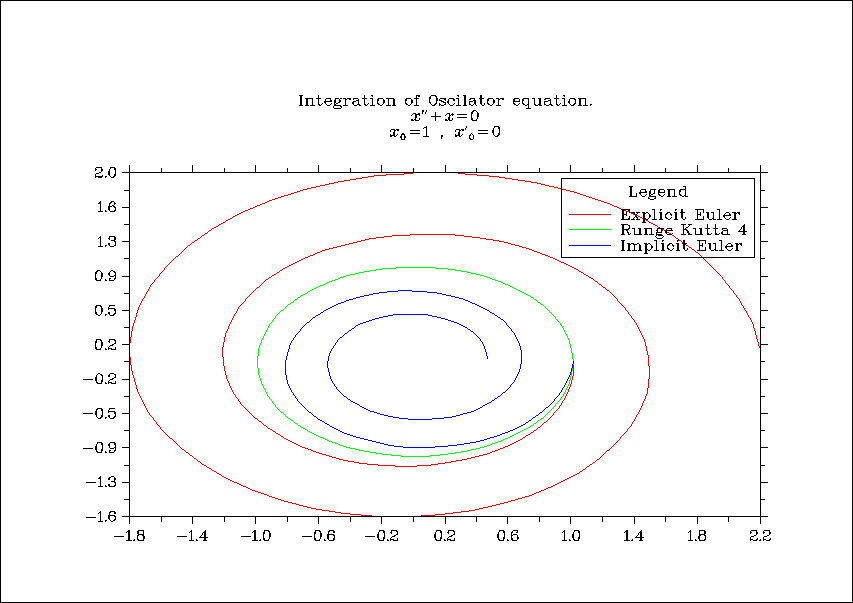
\includegraphics[scale=0.35]{px.png}
			\caption{Mapa de fases}
		\end{center}
	\end{figure}

	\newpage
	
	\begin{figure}[h!]
		\begin{center}
			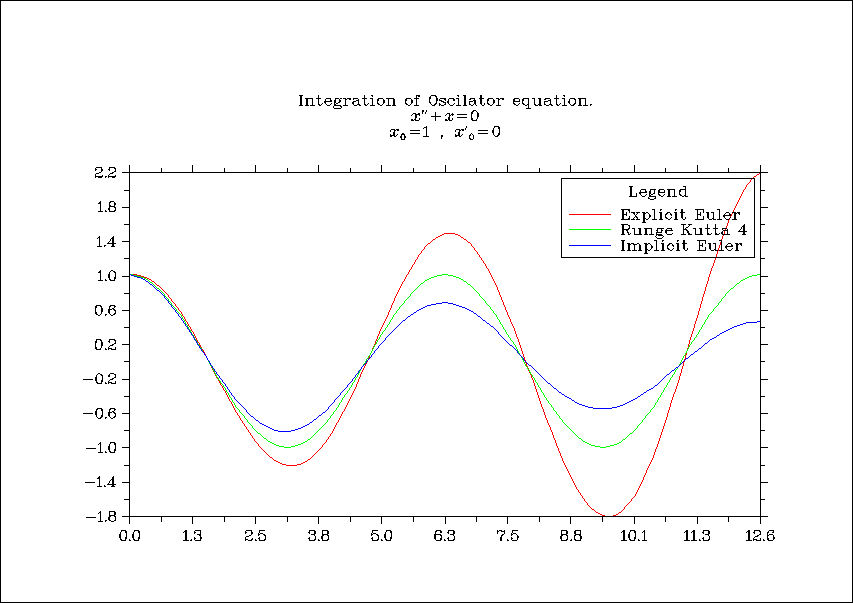
\includegraphics[scale=0.35]{xt.png}
			\caption{Posición respecto x}
		\end{center}
	\end{figure}

	En estas gráficas se observa que el comportamiento de la solución varía dependiendo del método numérico utilizado. Como se había adelantado en la descripción de cada uno de los métodos, para el Euler explícito la solución diverge, para el Euler implícito la converge a cero y para el Runge-Kutta de orden 4 la solución converge a un valor no nulo, siendo estas dos últimas soluciones estables.
	
	En el caso del Euler explícito, las condiciones iniciales definidas para este problema hacen que el problema sea inestable. Si se quisiese buscar la estabilidad, se debería hacer tender a cero $\Delta t$ teniendo en cuenta como es la región de estabilidad de este método. Con ello se conseguiría encontrarse en la frontera de dicha región por lo que el problema pasaría a ser condicionalmente estable. De todos modos, debido a que $\Delta t$ nunca puede ser igual a cero solo se podría acercar al punto anteriormente descrito.
	
	Para el Euler explícito, la solución es estable pero va decayendo continuamente. La región de estabilidad de este método es la inversa de la del método de Euler, por lo que en este caso con las condiciones iniciales de antes nos encontramos en la región de estabilidad del método haciendo que este sea incondicionalmente estable.
	
	Para el último caso, Runge-Kutta de orden 4, la solución converge a un valor determinado distinto de cero.
	
	Con el objetivo de conseguir un resultado ajustado a la realidad se debe emplear un esquema numérico que preserve el carácter de estabilidad, es decir, si el problema es estable se debe usar un esquema numérico estable y viceversa.
	
	Como el problema del oscilador armónico es un problema con autovalores imaginarios puros siempre se debe buscar encontrarse en la frontera de la región de estabilidad. En los casos de Euler explícito e implícito la parte de la frontera correspondiente al eje imaginario solo es el origen de coordenadas ($\Delta t=0s$) por lo que será un valor asintótico mientras que para el Runge-Kutta 4, la frontera pasa por varios puntos del eje imaginario.
	
	De los diferentes comportamientos se puede deducir que es necesario usar un método numérico con un error de integración muy bajo ya que para el estudio de órbitas se analizarán períodos de temporales altos donde el error se irá acumulado. De este hecho salen el decaimiento y la divergencia de los métodos Euler implícito y explícito, respectivamente. Además, siempre hay que tener muy presente el fenómeno físico que se está analizado así como sus condiciones. En el ejemplo del decaimiento, se puede llegar a pensar que es propio de alguna cuestión física (resistencia aerodinámica de la atmósfera) si no se conoce el problema objeto de estudio. Sin embargo, como se sabe que dicho movimiento es conservativo, la solución a obtener no puede decaer con el tiempo por lo que se llega a la conclusión de que este hecho ocurre debido a la acumulación de errores en la integración temporal.
	
	\section{Problema de los N cuerpos}
	
	La ecuación del problema de los $N$ cuerpos es la mostrada a continuación.
	
	$$m_i \ddot{\vec{r_i}}=-G\sum_{j=1}^{N}m_im_j\frac{\vec{r}_j-\vec{r}_i}{|\vec{r}_j-\vec{r}_i|^3}$$
	$$\vec{r}_i(0)=\vec{r}_{i0}$$
	$$\vec{v}_i(0)=\vec{v}_{i0}$$
	
	En este caso se ha decidido utilizar condiciones iniciales aleatorias para ver el comportamiento de un sistema al azar, teniendo en cuenta que este problema físico es un sistema caótico para $N>2$.
	
	En este caso, la transformación del sistema de $3N$ ecuaciones de orden dos se transforma en un sistema de $6N$ ecuaciones de orden unidad.
	
	\[
	U=\left[\begin{array}{c}
	m_{1}\\
	\vdots\\
	x_{1}\\
	y_{1}\\
	z_{1}\\
	v_{x1}\\
	v_{y1}\\
	v_{z1}\\
	\vdots
	\end{array}\right]\rightarrow\frac{dU}{dt}=\left[\begin{array}{c}
	0\\
	\vdots\\
	v_{x1}\\
	v_{y1}\\
	v_{z1}\\
	a_{x1}\\
	a_{y1}\\
	a_{z1}\\
	\vdots
	\end{array}\right]=F(U,t)
	\]
	
	\begin{center}
		Donde
	\end{center}
	$$a_i=-G\sum_{j=1}^{N}m_j\frac{\vec{r}_j-\vec{r}_i}{|\vec{r}_j-\vec{r}_i|^3}$$
	
	Adicionalmente se han añadido las $N$ masas en primeras $N$ componentes del vector de estado para facilitar su uso mediante punteros.
	
	El código que implementa el método numérico Runge-Kutta 4 aplicado a este problema empieza asignando unas condiciones iniciales aleatorias, cada una con unos órdenes de magnitud adecuados al caso. Además se anulan las posiciones y velocidades iniciales de la componente $z$ para que el movimiento se encuentre contenido en el plano $x,y$.
	
	Mediante la subrutina \textit{calc\_n\_bodies} que tiene como argumentos las condiciones iniciales, el dominio temporal y vector de estado U, y que a su vez contiene la subrutina \textit{cauchy\_problem} con los argumentos definidos previamente (el operador diferencial es en este caso \textit{f\_n\_bodies} y el esquema numérico, un Runge-Kutta 4 como se ha mencionado) se obtiene la solución del problema. La representación gráfica de las órbitas en el plano $x,y$ se muestra a continuación en las siguientes figuras.
	
	\newpage
	
	\begin{figure}[h!]
		\begin{center}
			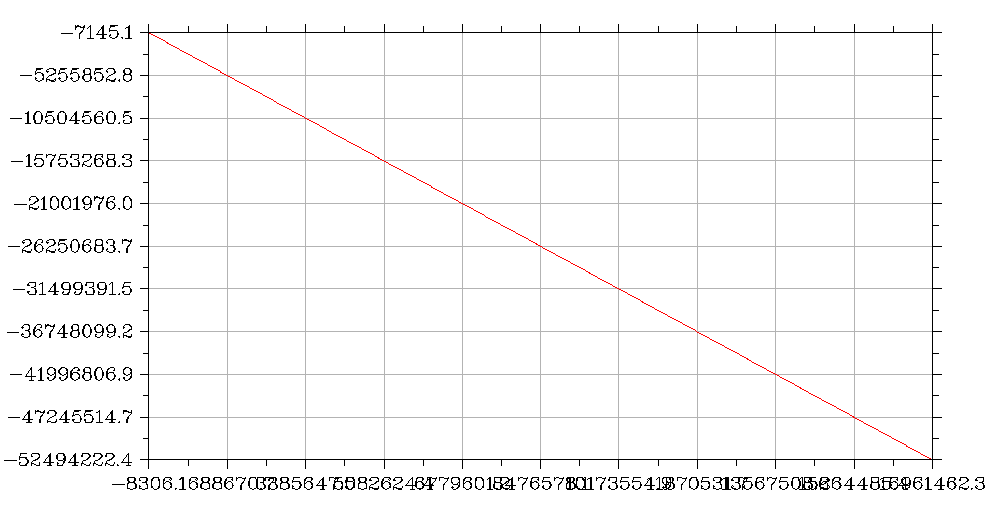
\includegraphics[scale=0.45]{nbodies1.png}
			\caption{Órbita del cuerpo 1 para el problema de 800 cuerpos}
		\end{center}
	\end{figure}

	\begin{figure}[h!]
		\begin{center}
			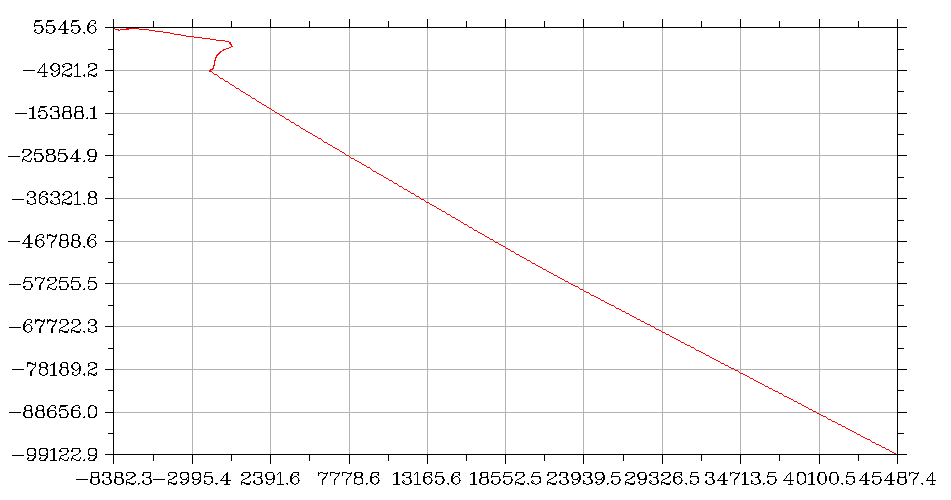
\includegraphics[scale=0.45]{nbodies2.png}
			\caption{Órbita del cuerpo 2 para el problema de 800 cuerpos}
		\end{center}
	\end{figure}

	\newpage

	\begin{figure}[h!]
		\begin{center}
			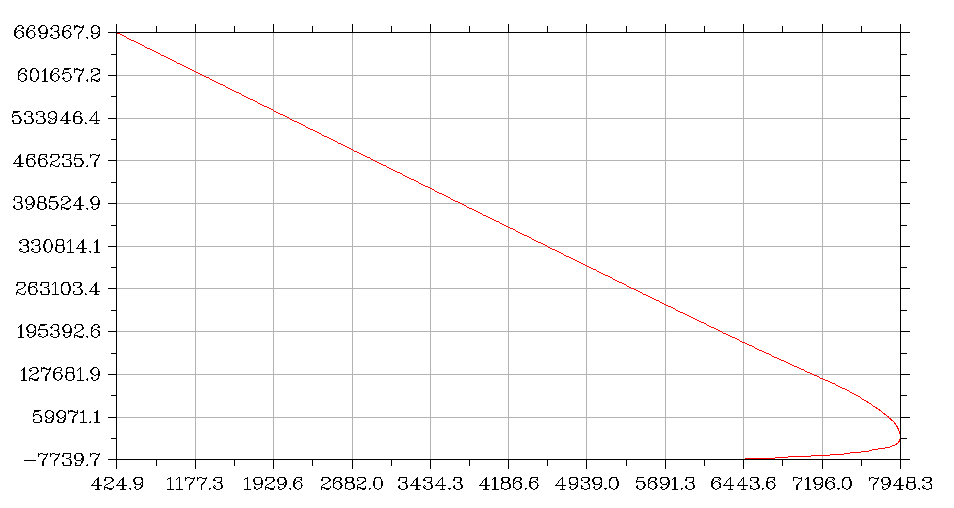
\includegraphics[scale=0.45]{nbodies3.png}
			\caption{Órbita del cuerpo 3 para el problema de 800 cuerpos}
		\end{center}
	\end{figure}

	\begin{figure}[h!]
		\begin{center}
			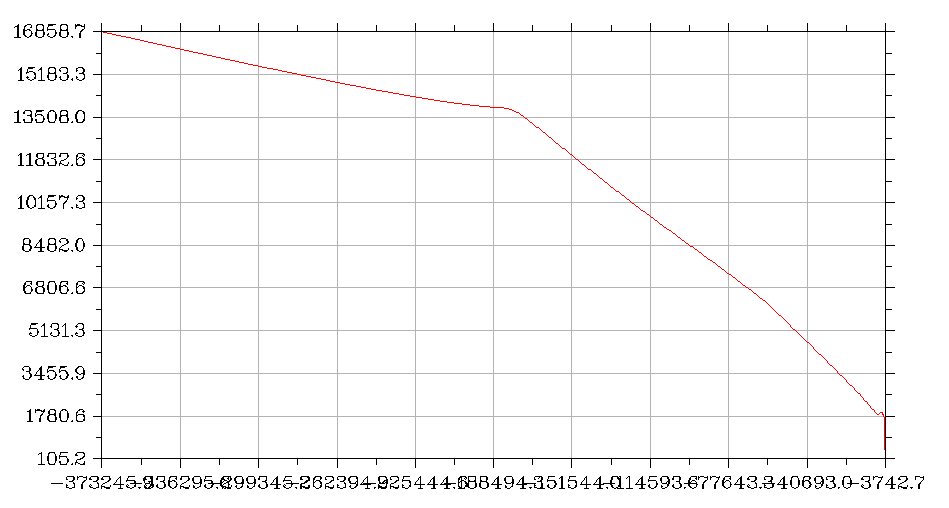
\includegraphics[scale=0.45]{nbodies4.png}
			\caption{Órbita del cuerpo 4 para el problema de 800 cuerpos}
		\end{center}
	\end{figure}

	En estas imágenes se han seleccionado los movimientos de ciertos cuerpos que muestran varios de los comportamientos que se pueden encontrar en el problema de los N cuerpos. Estas curvas tienden a escapar de forma asintótica por lo que de la forma de estas se puede deducir el carácter inestable del sistema.
	
	\newpage
	
	\section{Estabilidad de los puntos de Lagrange del sistema Tierra-Luna}
	
	Para un sistema de dos cuerpos masivos, los puntos de Lagrange son cinco puntos alrededor de los cuales un tercer objeto no masivo puede orbitar manteniendo la posición relativa respecto a los otros dos cuerpos masivos. Para el estudio de la estabilidad de dichos puntos se ha realizado un código en FORTRAN usando el paradigma de programación orientada a objetos. Este paradigma se suele emplear cuando la complejidad de los objetos que se quiere estudiar es alta (por ejemplo, un satélite compuesto por varios subsistemas y estos a su vez por multiples componentes) en contraposición con la programación funcional, usada cuando el objeto a modelar es simple. Este no es el caso que nos concierne pero se ha usado este paradigma a modo ilustrativo.
	
	El código utiliza un módulo para el cálculo de los puntos de Lagrange y otro para el uso de objetos, además de los módulos empleados anteriormente para en l problema de los N cuerpos y el problema de Cauchy. Las órbitas de la Tierra, la Luna y cada uno de los puntos de Lagrange alrededor del centro de masas de ambos se muestran gráficamente en las figuras que se muestran a continuación.
	
	\begin{figure}[h!]
		\begin{center}
			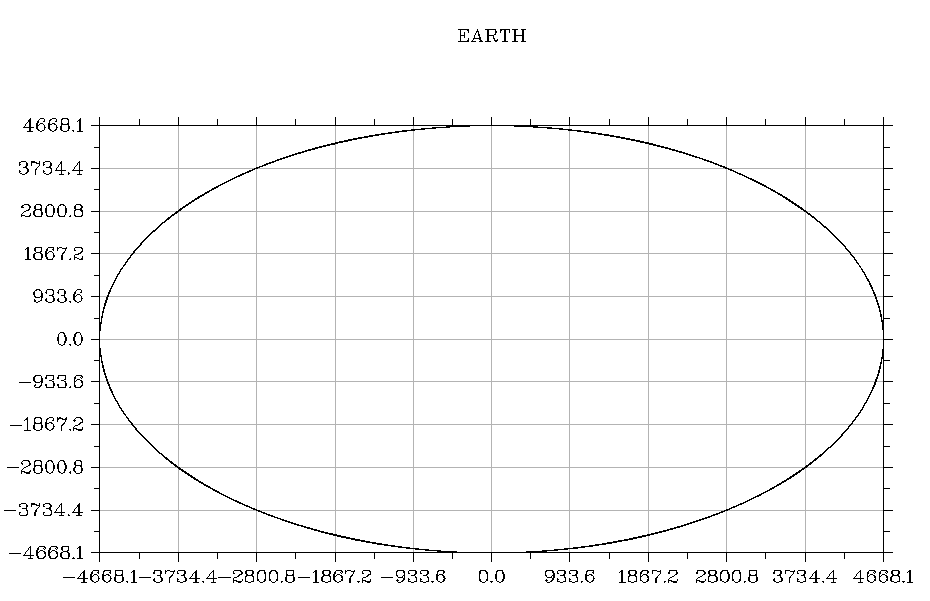
\includegraphics[scale=0.4]{earth.png}
			\caption{Órbita de la Tierra alrededor del centro de masas del sistema Tierra-Luna}
		\end{center}
	\end{figure}

	\begin{figure}[h!]
		\begin{center}
			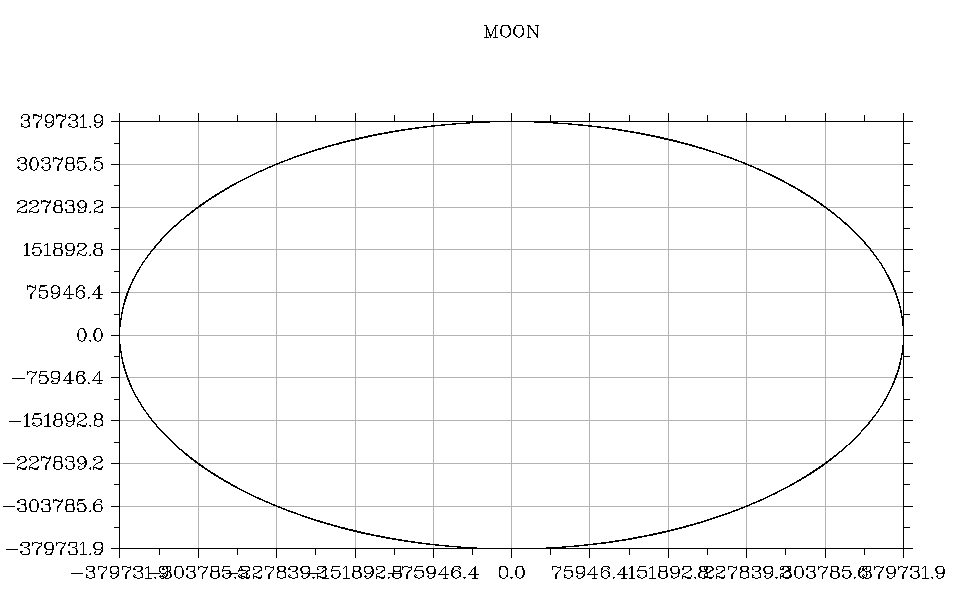
\includegraphics[scale=0.4]{moon.png}
			\caption{Órbita de la Luna alrededor del centro de masas del sistema Tierra-Luna}
		\end{center}
	\end{figure}

	\newpage

	\begin{figure}[h!]
		\begin{center}
			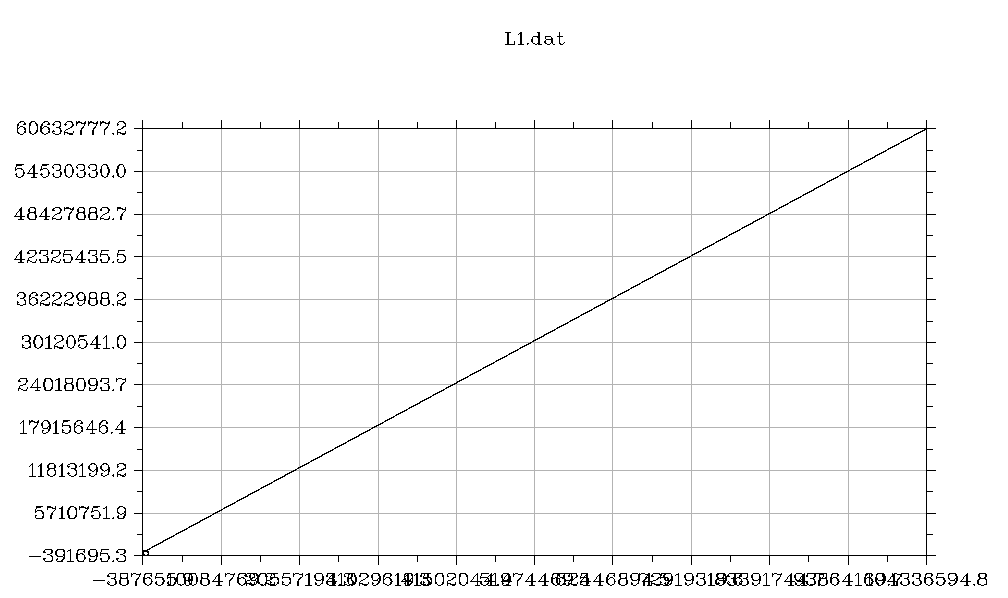
\includegraphics[scale=0.5]{l1.png}
			\caption{Órbita de punto L1 alrededor del centro de masas del sistema Tierra-Luna}
		\end{center}
	\end{figure}

	\begin{figure}[h!]
		\begin{center}
			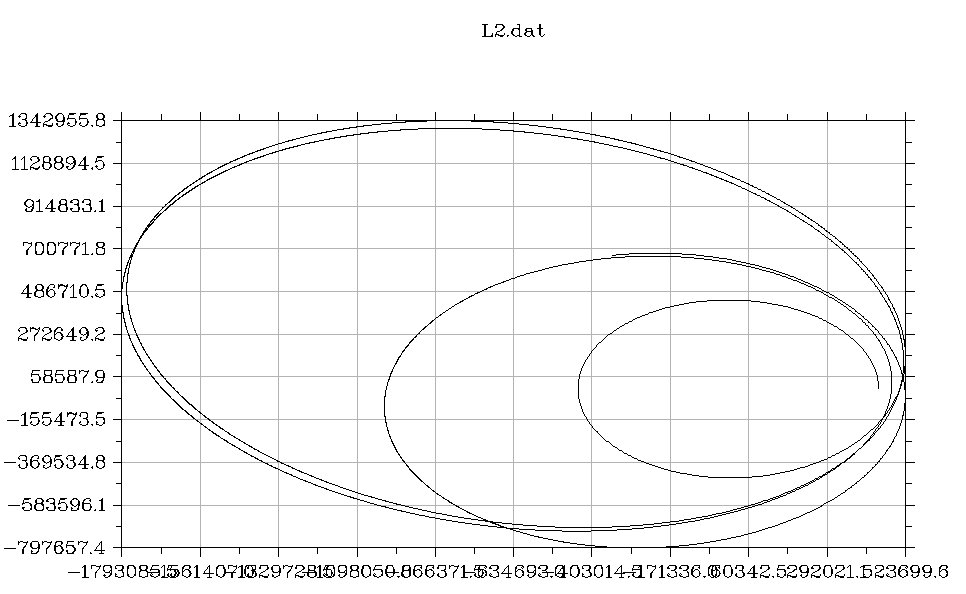
\includegraphics[scale=0.5]{l2.png}
			\caption{Órbita de punto L2 alrededor del centro de masas del sistema Tierra-Luna}
		\end{center}
	\end{figure}

	\newpage

	\begin{figure}[h!]
		\begin{center}
			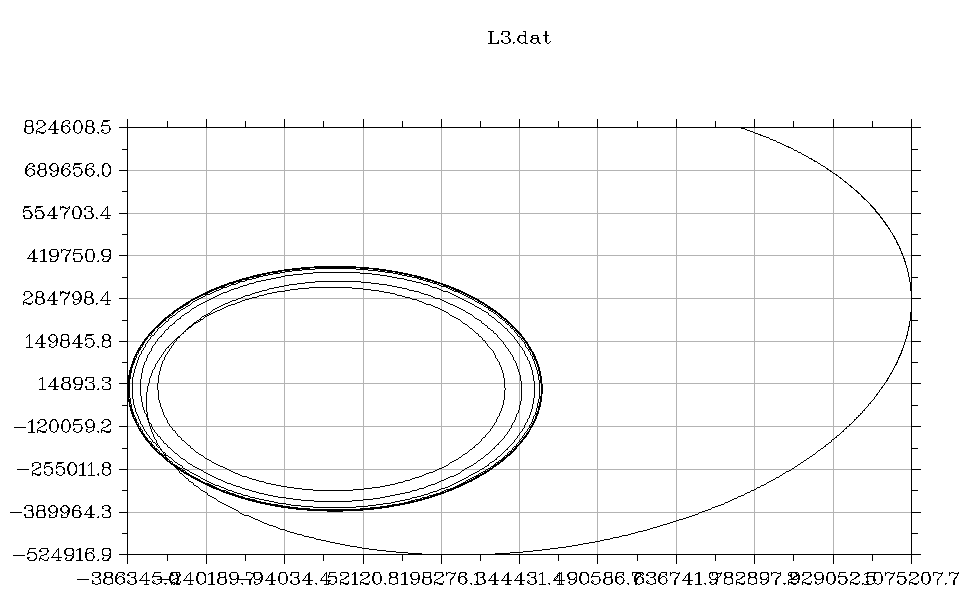
\includegraphics[scale=0.5]{l3.png}
			\caption{Órbita de punto L3 alrededor del centro de masas del sistema Tierra-Luna}
		\end{center}
	\end{figure}

	\begin{figure}[h!]
		\begin{center}
			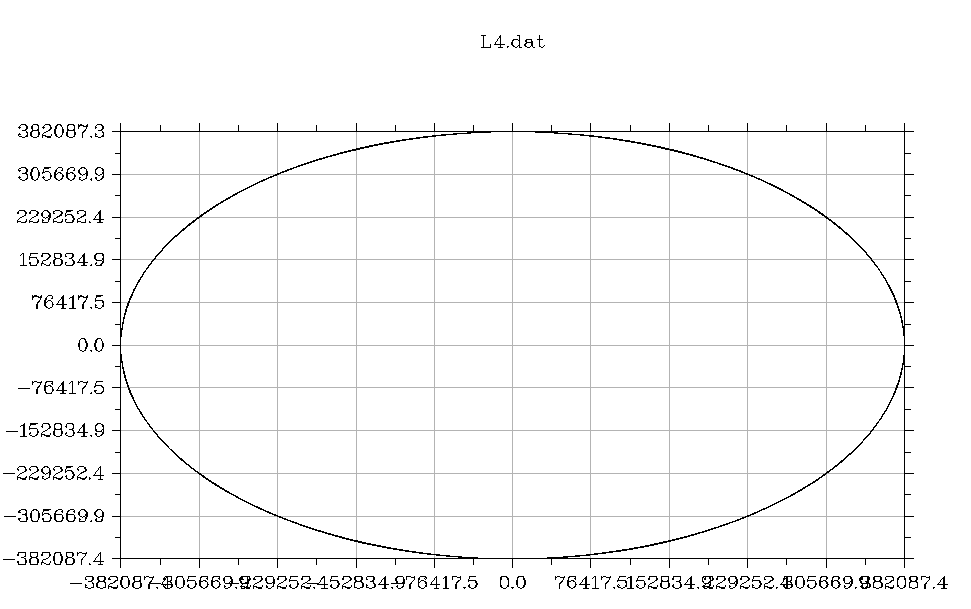
\includegraphics[scale=0.5]{l4.png}
			\caption{Órbita de punto L4 alrededor del centro de masas del sistema Tierra-Luna}
		\end{center}
	\end{figure}

	\newpage

	\begin{figure}[h!]
		\begin{center}
			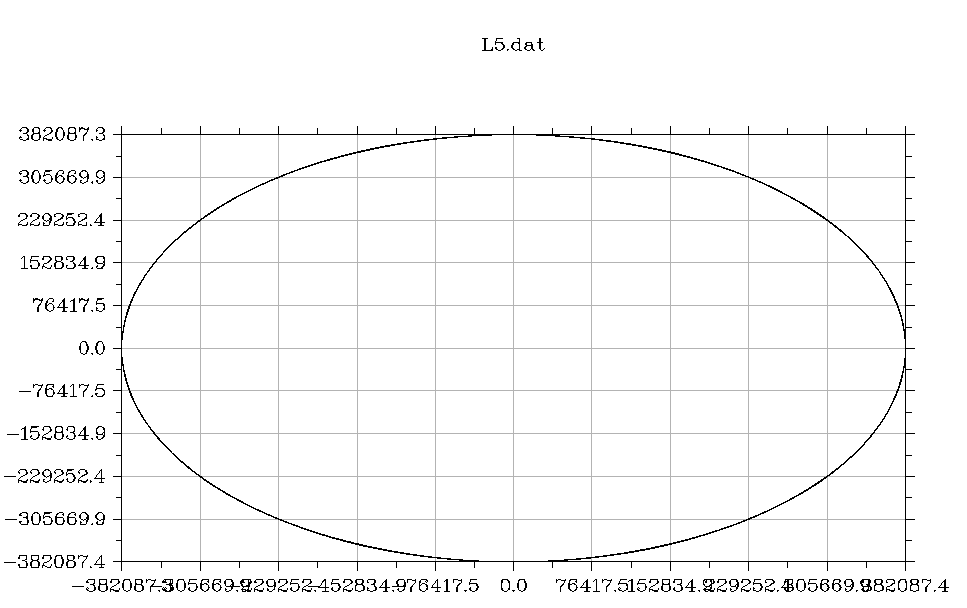
\includegraphics[scale=0.5]{l5.png}
			\caption{Órbita de punto L5 alrededor del centro de masas del sistema Tierra-Luna}
		\end{center}
	\end{figure}

	En estas gráficas se puede ver claramente el carácter de cada uno de los puntos. En la figura 10 se observa que el punto L1 es el más inestable de todos. Por otra parte, las soluciones de los puntos L2 y L3 también son inestables, tendiendo a infinito sus curvas aunque de una forma menos pronunciada que en el punto L1. Finalmente, se tiene los puntos L4 y L5 que son estables, estando todo acorde a la teoría.
	
	\newpage
	
	\section{Mapa de Poincaré}
	
	El mapa de Poincaré está compuesto por las proyecciones de las órbitas sobre un plano para diferentes valores de las condiciones iniciales. En el caso de este problema se van a realizar el mapa de Poincaré de los puntos L1 y L4 para las variaciones de las condiciones iniciales $x_0$ y $v_{y0}$.
	
	El código utiliza principalmente dos subrutinas anidadas: una que calcula el dominio temporal y las $\epsilon$ de las variaciones y otra dentro de esta que resuelve el problema de los tres cuerpos, calcula la intersección con el plano de Poincaré y genera las gráficas correspondientes. Estas figuras son las que se muestran a continuación.
	
	\begin{figure}[h!]
		\begin{center}
			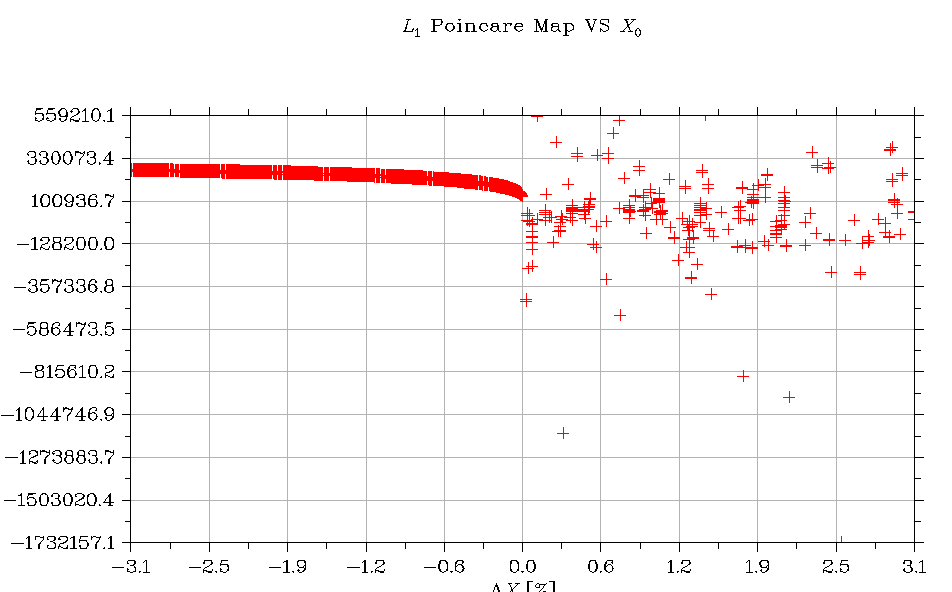
\includegraphics[scale=0.45]{p1.png}
			\caption{Mapa de Poincaré del punto L1 para variaciones de x0}
		\end{center}
	\end{figure}

	\begin{figure}[h!]
		\begin{center}
			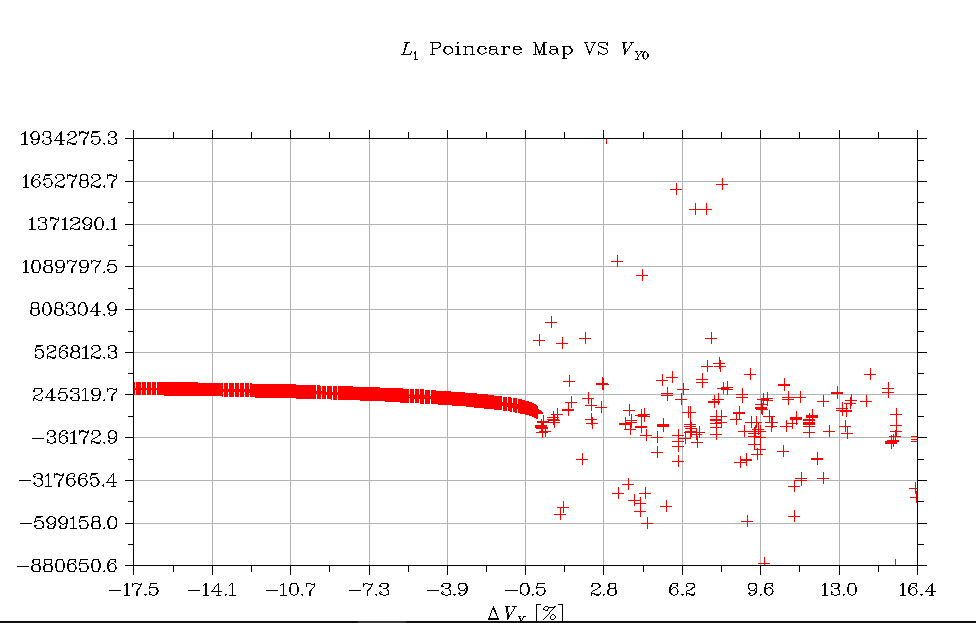
\includegraphics[scale=0.45]{p2.png}
			\caption{Mapa de Poincaré del punto L1 para variaciones de vy0}
		\end{center}
	\end{figure}

	\newpage

	\begin{figure}[h!]
		\begin{center}
			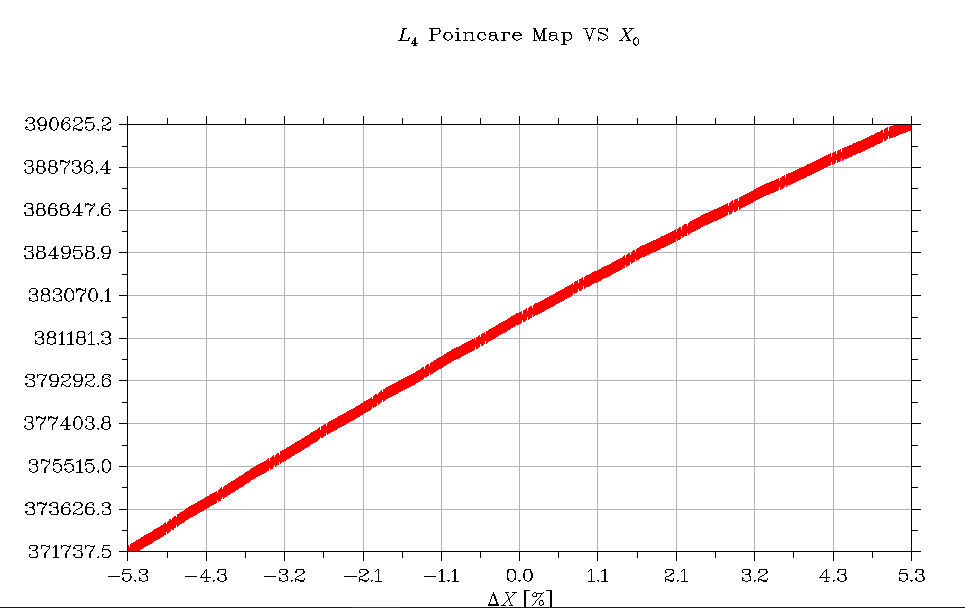
\includegraphics[scale=0.45]{p3.png}
			\caption{Mapa de Poincaré del punto L4 para variaciones de x0}
		\end{center}
	\end{figure}

	\begin{figure}[h!]
		\begin{center}
			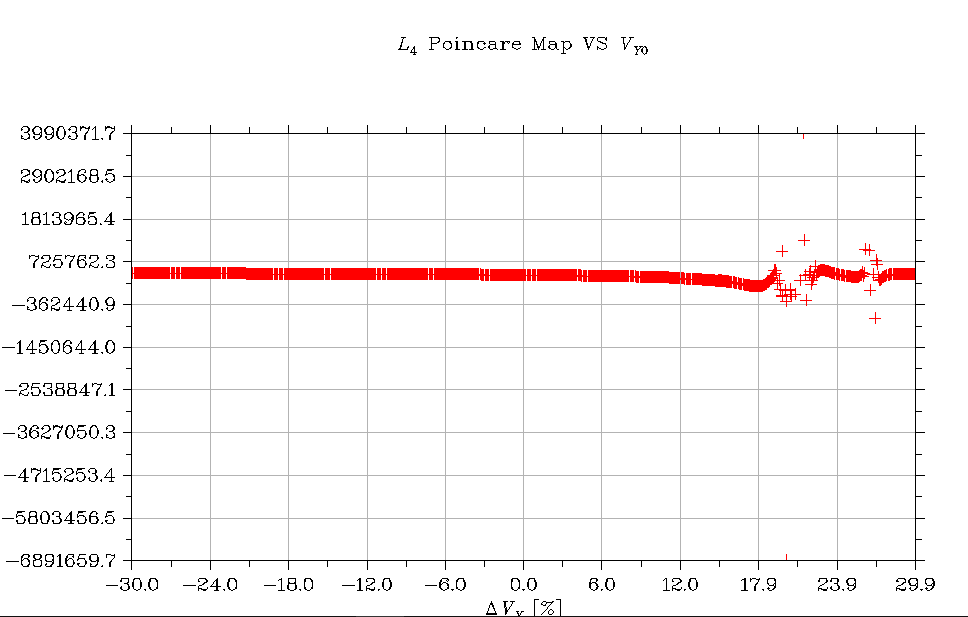
\includegraphics[scale=0.45]{p4.png}
			\caption{Mapa de Poincaré del punto L4 para variaciones de vy0}
		\end{center}
	\end{figure}
	
	En las figuras correspondientes al punto L1 se observa el carácter inestable ya que al aplicar variaciones en las condiciones iniciales se obtienen valores muy dispersos de este punto.
	
	Por otro lado, debido a que el punto L4 es estable, se observa como para variaciones de las condiciones iniciales no existen cambios de mayor orden de magnitud en el valor de este punto, a excepción de dos puntos para variaciones de la velocidad $v_{y0}$.
	
	\newpage
	
	\section{Interpolación de Richardson}
	
	Para la realización de este apartado se va a resolver un problema mediante la subrutina \textit{cauchy\_problem} con un dominio temporal, se resolverá el mismo problema para $\frac{\Delta t}{2}$ y también se hallará la solución a este mismo problema aplicando la extrapolación de Richardson. Posteriormente, se va a comprobar el error cometido con ambas aproximaciones respecto de la solución analítica. Para ello se ha usado un módulo que contiene una subrutina que calcula dicha interpolación, además de los módulos ya empleados anteriormente en la resolución de otros problemas de Cauchy. Finalmente se han representado el error cometido con la extrapolación de Richardson, los errores de cometidos con Cauchy y Richardson respecto a la solución analítica y el error de la interpolación de Richardson respecto a la solución real.
	
	\begin{figure}[h!]
		\begin{center}
			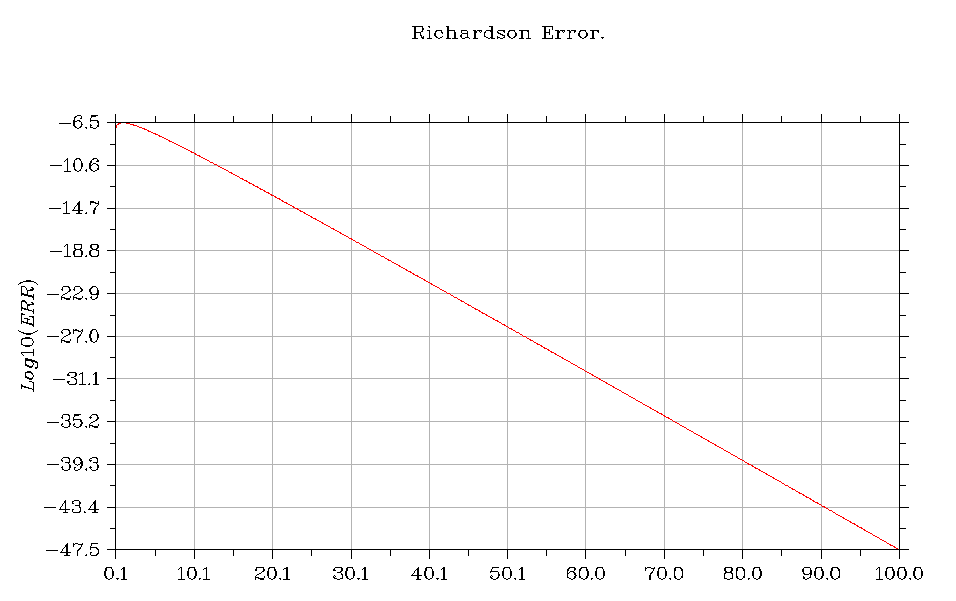
\includegraphics[scale=0.45]{richardson1.png}
			\caption{Error cometido con la extrapolación de Richardson}
		\end{center}
	\end{figure}

	\begin{figure}[h!]
		\begin{center}
			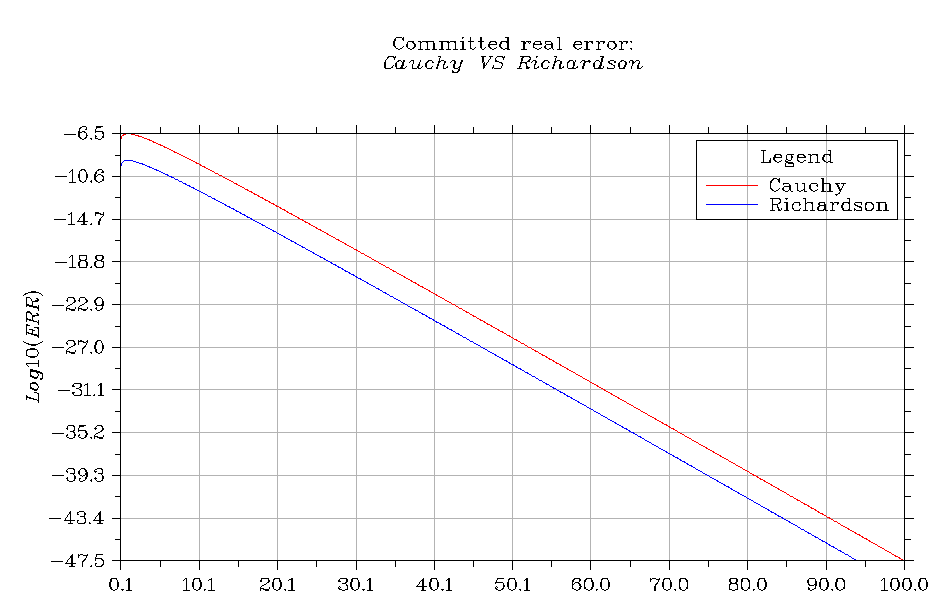
\includegraphics[scale=0.45]{richardson2.png}
			\caption{Error real de la extrapolación de Richardson y el problema de Cauchy}
		\end{center}
	\end{figure}

	\newpage

	\begin{figure}[h!]
		\begin{center}
			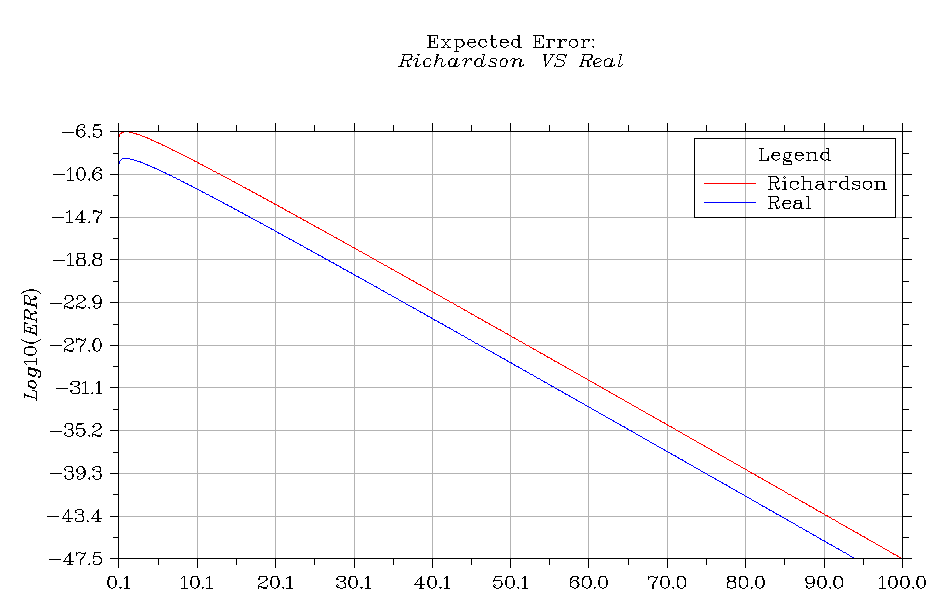
\includegraphics[scale=0.45]{richardson3.png}
			\caption{Error cometido con la extrapolación de Richardson respecto a la solución analítica}
		\end{center}
	\end{figure}
	
\end{document}